% Options for packages loaded elsewhere
\PassOptionsToPackage{unicode}{hyperref}
\PassOptionsToPackage{hyphens}{url}
\PassOptionsToPackage{dvipsnames,svgnames,x11names}{xcolor}
%
\documentclass[
  letterpaper,
  DIV=11,
  numbers=noendperiod]{scrartcl}

\usepackage{amsmath,amssymb}
\usepackage{iftex}
\ifPDFTeX
  \usepackage[T1]{fontenc}
  \usepackage[utf8]{inputenc}
  \usepackage{textcomp} % provide euro and other symbols
\else % if luatex or xetex
  \usepackage{unicode-math}
  \defaultfontfeatures{Scale=MatchLowercase}
  \defaultfontfeatures[\rmfamily]{Ligatures=TeX,Scale=1}
\fi
\usepackage{lmodern}
\ifPDFTeX\else  
    % xetex/luatex font selection
\fi
% Use upquote if available, for straight quotes in verbatim environments
\IfFileExists{upquote.sty}{\usepackage{upquote}}{}
\IfFileExists{microtype.sty}{% use microtype if available
  \usepackage[]{microtype}
  \UseMicrotypeSet[protrusion]{basicmath} % disable protrusion for tt fonts
}{}
\makeatletter
\@ifundefined{KOMAClassName}{% if non-KOMA class
  \IfFileExists{parskip.sty}{%
    \usepackage{parskip}
  }{% else
    \setlength{\parindent}{0pt}
    \setlength{\parskip}{6pt plus 2pt minus 1pt}}
}{% if KOMA class
  \KOMAoptions{parskip=half}}
\makeatother
\usepackage{xcolor}
\setlength{\emergencystretch}{3em} % prevent overfull lines
\setcounter{secnumdepth}{-\maxdimen} % remove section numbering
% Make \paragraph and \subparagraph free-standing
\makeatletter
\ifx\paragraph\undefined\else
  \let\oldparagraph\paragraph
  \renewcommand{\paragraph}{
    \@ifstar
      \xxxParagraphStar
      \xxxParagraphNoStar
  }
  \newcommand{\xxxParagraphStar}[1]{\oldparagraph*{#1}\mbox{}}
  \newcommand{\xxxParagraphNoStar}[1]{\oldparagraph{#1}\mbox{}}
\fi
\ifx\subparagraph\undefined\else
  \let\oldsubparagraph\subparagraph
  \renewcommand{\subparagraph}{
    \@ifstar
      \xxxSubParagraphStar
      \xxxSubParagraphNoStar
  }
  \newcommand{\xxxSubParagraphStar}[1]{\oldsubparagraph*{#1}\mbox{}}
  \newcommand{\xxxSubParagraphNoStar}[1]{\oldsubparagraph{#1}\mbox{}}
\fi
\makeatother

\usepackage{color}
\usepackage{fancyvrb}
\newcommand{\VerbBar}{|}
\newcommand{\VERB}{\Verb[commandchars=\\\{\}]}
\DefineVerbatimEnvironment{Highlighting}{Verbatim}{commandchars=\\\{\}}
% Add ',fontsize=\small' for more characters per line
\usepackage{framed}
\definecolor{shadecolor}{RGB}{241,243,245}
\newenvironment{Shaded}{\begin{snugshade}}{\end{snugshade}}
\newcommand{\AlertTok}[1]{\textcolor[rgb]{0.68,0.00,0.00}{#1}}
\newcommand{\AnnotationTok}[1]{\textcolor[rgb]{0.37,0.37,0.37}{#1}}
\newcommand{\AttributeTok}[1]{\textcolor[rgb]{0.40,0.45,0.13}{#1}}
\newcommand{\BaseNTok}[1]{\textcolor[rgb]{0.68,0.00,0.00}{#1}}
\newcommand{\BuiltInTok}[1]{\textcolor[rgb]{0.00,0.23,0.31}{#1}}
\newcommand{\CharTok}[1]{\textcolor[rgb]{0.13,0.47,0.30}{#1}}
\newcommand{\CommentTok}[1]{\textcolor[rgb]{0.37,0.37,0.37}{#1}}
\newcommand{\CommentVarTok}[1]{\textcolor[rgb]{0.37,0.37,0.37}{\textit{#1}}}
\newcommand{\ConstantTok}[1]{\textcolor[rgb]{0.56,0.35,0.01}{#1}}
\newcommand{\ControlFlowTok}[1]{\textcolor[rgb]{0.00,0.23,0.31}{\textbf{#1}}}
\newcommand{\DataTypeTok}[1]{\textcolor[rgb]{0.68,0.00,0.00}{#1}}
\newcommand{\DecValTok}[1]{\textcolor[rgb]{0.68,0.00,0.00}{#1}}
\newcommand{\DocumentationTok}[1]{\textcolor[rgb]{0.37,0.37,0.37}{\textit{#1}}}
\newcommand{\ErrorTok}[1]{\textcolor[rgb]{0.68,0.00,0.00}{#1}}
\newcommand{\ExtensionTok}[1]{\textcolor[rgb]{0.00,0.23,0.31}{#1}}
\newcommand{\FloatTok}[1]{\textcolor[rgb]{0.68,0.00,0.00}{#1}}
\newcommand{\FunctionTok}[1]{\textcolor[rgb]{0.28,0.35,0.67}{#1}}
\newcommand{\ImportTok}[1]{\textcolor[rgb]{0.00,0.46,0.62}{#1}}
\newcommand{\InformationTok}[1]{\textcolor[rgb]{0.37,0.37,0.37}{#1}}
\newcommand{\KeywordTok}[1]{\textcolor[rgb]{0.00,0.23,0.31}{\textbf{#1}}}
\newcommand{\NormalTok}[1]{\textcolor[rgb]{0.00,0.23,0.31}{#1}}
\newcommand{\OperatorTok}[1]{\textcolor[rgb]{0.37,0.37,0.37}{#1}}
\newcommand{\OtherTok}[1]{\textcolor[rgb]{0.00,0.23,0.31}{#1}}
\newcommand{\PreprocessorTok}[1]{\textcolor[rgb]{0.68,0.00,0.00}{#1}}
\newcommand{\RegionMarkerTok}[1]{\textcolor[rgb]{0.00,0.23,0.31}{#1}}
\newcommand{\SpecialCharTok}[1]{\textcolor[rgb]{0.37,0.37,0.37}{#1}}
\newcommand{\SpecialStringTok}[1]{\textcolor[rgb]{0.13,0.47,0.30}{#1}}
\newcommand{\StringTok}[1]{\textcolor[rgb]{0.13,0.47,0.30}{#1}}
\newcommand{\VariableTok}[1]{\textcolor[rgb]{0.07,0.07,0.07}{#1}}
\newcommand{\VerbatimStringTok}[1]{\textcolor[rgb]{0.13,0.47,0.30}{#1}}
\newcommand{\WarningTok}[1]{\textcolor[rgb]{0.37,0.37,0.37}{\textit{#1}}}

\providecommand{\tightlist}{%
  \setlength{\itemsep}{0pt}\setlength{\parskip}{0pt}}\usepackage{longtable,booktabs,array}
\usepackage{calc} % for calculating minipage widths
% Correct order of tables after \paragraph or \subparagraph
\usepackage{etoolbox}
\makeatletter
\patchcmd\longtable{\par}{\if@noskipsec\mbox{}\fi\par}{}{}
\makeatother
% Allow footnotes in longtable head/foot
\IfFileExists{footnotehyper.sty}{\usepackage{footnotehyper}}{\usepackage{footnote}}
\makesavenoteenv{longtable}
\usepackage{graphicx}
\makeatletter
\newsavebox\pandoc@box
\newcommand*\pandocbounded[1]{% scales image to fit in text height/width
  \sbox\pandoc@box{#1}%
  \Gscale@div\@tempa{\textheight}{\dimexpr\ht\pandoc@box+\dp\pandoc@box\relax}%
  \Gscale@div\@tempb{\linewidth}{\wd\pandoc@box}%
  \ifdim\@tempb\p@<\@tempa\p@\let\@tempa\@tempb\fi% select the smaller of both
  \ifdim\@tempa\p@<\p@\scalebox{\@tempa}{\usebox\pandoc@box}%
  \else\usebox{\pandoc@box}%
  \fi%
}
% Set default figure placement to htbp
\def\fps@figure{htbp}
\makeatother
% definitions for citeproc citations
\NewDocumentCommand\citeproctext{}{}
\NewDocumentCommand\citeproc{mm}{%
  \begingroup\def\citeproctext{#2}\cite{#1}\endgroup}
\makeatletter
 % allow citations to break across lines
 \let\@cite@ofmt\@firstofone
 % avoid brackets around text for \cite:
 \def\@biblabel#1{}
 \def\@cite#1#2{{#1\if@tempswa , #2\fi}}
\makeatother
\newlength{\cslhangindent}
\setlength{\cslhangindent}{1.5em}
\newlength{\csllabelwidth}
\setlength{\csllabelwidth}{3em}
\newenvironment{CSLReferences}[2] % #1 hanging-indent, #2 entry-spacing
 {\begin{list}{}{%
  \setlength{\itemindent}{0pt}
  \setlength{\leftmargin}{0pt}
  \setlength{\parsep}{0pt}
  % turn on hanging indent if param 1 is 1
  \ifodd #1
   \setlength{\leftmargin}{\cslhangindent}
   \setlength{\itemindent}{-1\cslhangindent}
  \fi
  % set entry spacing
  \setlength{\itemsep}{#2\baselineskip}}}
 {\end{list}}
\usepackage{calc}
\newcommand{\CSLBlock}[1]{\hfill\break\parbox[t]{\linewidth}{\strut\ignorespaces#1\strut}}
\newcommand{\CSLLeftMargin}[1]{\parbox[t]{\csllabelwidth}{\strut#1\strut}}
\newcommand{\CSLRightInline}[1]{\parbox[t]{\linewidth - \csllabelwidth}{\strut#1\strut}}
\newcommand{\CSLIndent}[1]{\hspace{\cslhangindent}#1}

\KOMAoption{captions}{tableheading}
\makeatletter
\@ifpackageloaded{caption}{}{\usepackage{caption}}
\AtBeginDocument{%
\ifdefined\contentsname
  \renewcommand*\contentsname{Table of contents}
\else
  \newcommand\contentsname{Table of contents}
\fi
\ifdefined\listfigurename
  \renewcommand*\listfigurename{List of Figures}
\else
  \newcommand\listfigurename{List of Figures}
\fi
\ifdefined\listtablename
  \renewcommand*\listtablename{List of Tables}
\else
  \newcommand\listtablename{List of Tables}
\fi
\ifdefined\figurename
  \renewcommand*\figurename{Figure}
\else
  \newcommand\figurename{Figure}
\fi
\ifdefined\tablename
  \renewcommand*\tablename{Table}
\else
  \newcommand\tablename{Table}
\fi
}
\@ifpackageloaded{float}{}{\usepackage{float}}
\floatstyle{ruled}
\@ifundefined{c@chapter}{\newfloat{codelisting}{h}{lop}}{\newfloat{codelisting}{h}{lop}[chapter]}
\floatname{codelisting}{Listing}
\newcommand*\listoflistings{\listof{codelisting}{List of Listings}}
\makeatother
\makeatletter
\makeatother
\makeatletter
\@ifpackageloaded{caption}{}{\usepackage{caption}}
\@ifpackageloaded{subcaption}{}{\usepackage{subcaption}}
\makeatother

\usepackage{bookmark}

\IfFileExists{xurl.sty}{\usepackage{xurl}}{} % add URL line breaks if available
\urlstyle{same} % disable monospaced font for URLs
\hypersetup{
  pdftitle={Timeline check in},
  pdfauthor={Nina, Kelsey, Sofia},
  colorlinks=true,
  linkcolor={blue},
  filecolor={Maroon},
  citecolor={Blue},
  urlcolor={Blue},
  pdfcreator={LaTeX via pandoc}}


\title{Timeline check in}
\author{Nina, Kelsey, Sofia}
\date{2026-05-22}

\begin{document}
\maketitle


\begin{Shaded}
\begin{Highlighting}[]
\CommentTok{\# data wrangling and visualization}
\FunctionTok{library}\NormalTok{(tidyverse)}

\CommentTok{\# allows file paths to work across computers}
\FunctionTok{library}\NormalTok{(here)}

\CommentTok{\# formatting axis labels}
\FunctionTok{library}\NormalTok{(scales)}

\CommentTok{\# working with dates}
\FunctionTok{library}\NormalTok{(lubridate)}

\CommentTok{\# combining plots}
\FunctionTok{library}\NormalTok{(patchwork)}
\end{Highlighting}
\end{Shaded}

\begin{Shaded}
\begin{Highlighting}[]
\CommentTok{\# read in bird survey data}
\NormalTok{birds }\OtherTok{\textless{}{-}} \FunctionTok{read.csv}\NormalTok{(}\FunctionTok{here}\NormalTok{(}\StringTok{"data"}\NormalTok{, }\StringTok{"birds.csv"}\NormalTok{))}

\CommentTok{\# read in NOAA weather data}
\NormalTok{weather }\OtherTok{\textless{}{-}} \FunctionTok{read.csv}\NormalTok{(}\FunctionTok{here}\NormalTok{(}\StringTok{"data"}\NormalTok{, }\StringTok{"NOAA\_daily\_summaries.csv"}\NormalTok{))}
\end{Highlighting}
\end{Shaded}

\section{Ideas for analysis and
background}\label{ideas-for-analysis-and-background}

\subsection{Research Questions}\label{research-questions}

\begin{itemize}
\tightlist
\item
  What is the effect of previous month's precipitation on total monthly
  waterfowl abundance at NCOS?
\item
  How does total waterfowl abundance vary through time at NCOS?
\item
  Are there seasonal patterns in waterfowl abundance and precipitation
  at NCOS?
\end{itemize}

\subsection{Relevance}\label{relevance}

\textbf{Relevance to NCOS:} NCOS is a restored coastal wetland in Santa
Barbara, CA. Understanding what drives waterfowl abundance at this site
helps evaluate whether restoration efforts are creating suitable habitat
conditions for migratory and resident waterbirds.

\textbf{Relevance to other systems:} Precipitation-abundance
relationships in waterfowl are relevant to other California estuaries
and coastal wetlands, where water availability similarly structures
habitat quality. Findings from NCOS can inform management decisions at
comparable restored wetland systems throughout the region.

\textbf{Relevance to understanding the organisms and physical
processes:} Waterfowl are strongly tied to wetland hydrology;
precipitation influences water depth, food availability, and habitat
extent, all of which affect where and when birds concentrate (Kahara et
al. 2021; Stenzel and Page 2011). Understanding how rainfall patterns
shape waterfowl abundance contributes to broader knowledge of how
climate variability affects waterbird communities.

\subsection{Planned Analysis}\label{planned-analysis}

We plan to explore the relationship between lagged monthly precipitation
and total monthly waterfowl abundance using a scatter plot and linear
regression. We will also compare seasonal totals of both variables to
assess whether seasonal patterns align across water years 2020--2025.

\subsection{Citations}\label{citations}

\begin{itemize}
\item
  \textbf{Habitat quality and drought effects on breeding mallard and
  other waterfowl populations in California, USA} (Kahara et al. 2021):
  This report shows how drought impacts habitat quality which in turn
  impacts waterfowl population. This is relevant to our study because we
  are looking at how precipitation impacts waterfowl abundance.
  Precipitation is a factor for drought.
\item
  \textbf{Forecasting waterfowl population dynamics under climate change
  -- Does the spatial variation of density dependence and environmental
  effects matter?} (Zhao et al. 2016): This report found that due to
  climate change, Mallard density is predicted to decline. One of the
  climate variables they examine is precipitation. This is relevant to
  our study because we are looking at the effects of precipitation on
  waterfowl. Their modelling is similar to what we are retroactively
  looking at.
\item
  \textbf{The effect of climate change on optimal wetlands and waterfowl
  management in Western Canada} (Withey and Kooten 2011): This paper is
  relevant to our study because they are focusing on how climate change
  variables such as precipitation and temperature changes will affect
  wetland habitats. This is where waterbirds live and precipitation
  affects the quality of the habitat.
\item
  \textbf{Trends in abundance of wintering waterbirds relative to
  rainfall patterns at a central California estuary, 1972-2015} (Stenzel
  and Page 2011): This paper finds that there is a relationship between
  waterbirds and rainfall. They find that there is typically a negative
  relationship between the two, and that the relationship is stronger
  when looking at rainfall in the current year than in previous years.
  This is relevant to our study because we are looking at the
  relationship between waterfowl abundance and precipitation as well.
\end{itemize}

\section{Preliminary code for
analyses}\label{preliminary-code-for-analyses}

\subsection{Cleaning Data}\label{cleaning-data}

\begin{Shaded}
\begin{Highlighting}[]
\NormalTok{birds\_clean }\OtherTok{\textless{}{-}}\NormalTok{ birds }\SpecialCharTok{|\textgreater{}}
  \CommentTok{\# convert observation date to date format}
  \FunctionTok{mutate}\NormalTok{(}
    \AttributeTok{observation\_date =} \FunctionTok{ymd}\NormalTok{(observation\_date),}

    \CommentTok{\# create monthly grouping variable}
    \AttributeTok{month =} \FunctionTok{floor\_date}\NormalTok{(observation\_date,}
                       \AttributeTok{unit =} \StringTok{"month"}\NormalTok{)}
\NormalTok{  ) }\SpecialCharTok{|\textgreater{}}

  \CommentTok{\# filter to only include waterfowl observations}
  \FunctionTok{filter}\NormalTok{(}
\NormalTok{    e\_bird\_group }\SpecialCharTok{==} \StringTok{"Waterfowl"}\NormalTok{,}

    \CommentTok{\# remove repeat observations}
\NormalTok{    repeat\_observation }\SpecialCharTok{==} \StringTok{"No"}\NormalTok{,}

    \CommentTok{\# keep observations within study period}
\NormalTok{    observation\_date }\SpecialCharTok{\textgreater{}} \FunctionTok{ymd}\NormalTok{(}\StringTok{"2019{-}09{-}30"}\NormalTok{),}
\NormalTok{    observation\_date }\SpecialCharTok{\textless{}} \FunctionTok{ymd}\NormalTok{(}\StringTok{"2025{-}10{-}01"}\NormalTok{)}
\NormalTok{  )}
\end{Highlighting}
\end{Shaded}

\begin{Shaded}
\begin{Highlighting}[]
\NormalTok{weather\_clean }\OtherTok{\textless{}{-}}\NormalTok{ weather }\SpecialCharTok{|\textgreater{}} 
  
  \CommentTok{\# convert date column to date format}
  \FunctionTok{mutate}\NormalTok{(}
    \AttributeTok{DATE =} \FunctionTok{ymd}\NormalTok{(DATE),}
    
    \CommentTok{\# create monthly grouping variable}
    \AttributeTok{month =} \FunctionTok{floor\_date}\NormalTok{(DATE,}
                       \AttributeTok{unit =} \StringTok{"month"}\NormalTok{)}
\NormalTok{  ) }\SpecialCharTok{|\textgreater{}} 
  
  \CommentTok{\# filter to study period}
  \FunctionTok{filter}\NormalTok{(}
\NormalTok{    DATE }\SpecialCharTok{\textgreater{}} \FunctionTok{ymd}\NormalTok{(}\StringTok{"2019{-}09{-}30"}\NormalTok{),}
\NormalTok{    DATE }\SpecialCharTok{\textless{}} \FunctionTok{ymd}\NormalTok{(}\StringTok{"2025{-}10{-}01"}\NormalTok{)}
\NormalTok{  )}
\end{Highlighting}
\end{Shaded}

\subsection{Summaries}\label{summaries}

\begin{Shaded}
\begin{Highlighting}[]
\CommentTok{\# calculate total monthly precipitation}
\NormalTok{monthly\_precip }\OtherTok{\textless{}{-}}\NormalTok{ weather\_clean }\SpecialCharTok{|\textgreater{}} 
  
  \CommentTok{\# group observations by month}
  \FunctionTok{group\_by}\NormalTok{(month) }\SpecialCharTok{|\textgreater{}} 
  
  \CommentTok{\# sum precipitation within each month}
  \FunctionTok{summarize}\NormalTok{(}
    \AttributeTok{monthly\_prcp =} \FunctionTok{sum}\NormalTok{(PRCP, }\AttributeTok{na.rm =} \ConstantTok{TRUE}\NormalTok{),}
    
    \CommentTok{\# remove grouping after summarizing}
    \AttributeTok{.groups =} \StringTok{"drop"}
\NormalTok{  )}
\end{Highlighting}
\end{Shaded}

\begin{Shaded}
\begin{Highlighting}[]
\CommentTok{\# calculate monthly abundance by species}
\NormalTok{monthly\_waterfowl }\OtherTok{\textless{}{-}}\NormalTok{ birds\_clean }\SpecialCharTok{|\textgreater{}}

  \CommentTok{\# group by month and species}
  \FunctionTok{group\_by}\NormalTok{(month, species) }\SpecialCharTok{|\textgreater{}}

  \CommentTok{\# sum bird counts within each month}
  \FunctionTok{summarize}\NormalTok{(}
    \AttributeTok{abundance =} \FunctionTok{sum}\NormalTok{(count, }\AttributeTok{na.rm =} \ConstantTok{TRUE}\NormalTok{),}

    \CommentTok{\# remove grouping after summarizing}
    \AttributeTok{.groups =} \StringTok{"drop"}
\NormalTok{  ) }\SpecialCharTok{|\textgreater{}}

  \CommentTok{\# order species factor levels for stacked area plot}
  \CommentTok{\# arranging so similar colors are not adjacent in stack}
  \FunctionTok{mutate}\NormalTok{(}\AttributeTok{species =} \FunctionTok{factor}\NormalTok{(species, }\AttributeTok{levels =} \FunctionTok{c}\NormalTok{(}
    \StringTok{"Snow Goose"}\NormalTok{,}
    \StringTok{"Ross\textquotesingle{}s Goose"}\NormalTok{,}
    \StringTok{"Cackling Goose (Aleutian)"}\NormalTok{,}
    \StringTok{"Canada Goose"}\NormalTok{,}
    \StringTok{"Greater White{-}fronted Goose"}\NormalTok{,}
    \StringTok{"Ring{-}necked Duck"}\NormalTok{,}
    \StringTok{"Redhead"}\NormalTok{,}
    \StringTok{"Canvasback"}\NormalTok{,}
    \StringTok{"Ruddy Duck"}\NormalTok{,}
    \StringTok{"American Wigeon"}\NormalTok{,}
    \StringTok{"Blue{-}winged Teal"}\NormalTok{,}
    \StringTok{"Cinnamon Teal"}\NormalTok{,}
    \StringTok{"Northern Pintail"}\NormalTok{,}
    \StringTok{"Mallard"}\NormalTok{,}
    \StringTok{"Northern Shoveler"}\NormalTok{,}
    \StringTok{"Bufflehead"}\NormalTok{,}
    \StringTok{"Hooded Merganser"}\NormalTok{,}
    \StringTok{"Green{-}winged Teal"}\NormalTok{,}
    \StringTok{"Gadwall"}
\NormalTok{  )))}
\end{Highlighting}
\end{Shaded}

\begin{Shaded}
\begin{Highlighting}[]
\CommentTok{\# calculate total monthly waterfowl abundance}
\NormalTok{total\_monthly\_waterfowl }\OtherTok{\textless{}{-}}\NormalTok{ birds\_clean }\SpecialCharTok{|\textgreater{}} 
  
  \CommentTok{\# group by month}
  \FunctionTok{group\_by}\NormalTok{(month) }\SpecialCharTok{|\textgreater{}} 
  
  \CommentTok{\# sum all bird counts within each month}
  \FunctionTok{summarize}\NormalTok{(}
    \AttributeTok{total\_abundance =} \FunctionTok{sum}\NormalTok{(count, }\AttributeTok{na.rm =} \ConstantTok{TRUE}\NormalTok{),}
    
    \CommentTok{\# remove grouping after summarizing}
    \AttributeTok{.groups =} \StringTok{"drop"}
\NormalTok{  )}
\end{Highlighting}
\end{Shaded}

\subsection{Joining data}\label{joining-data}

\begin{Shaded}
\begin{Highlighting}[]
\CommentTok{\# join monthly bird abundance with monthly precipitation}
\NormalTok{bird\_weather\_monthly }\OtherTok{\textless{}{-}}\NormalTok{ total\_monthly\_waterfowl }\SpecialCharTok{|\textgreater{}}

  \CommentTok{\# join by month}
  \FunctionTok{left\_join}\NormalTok{(monthly\_precip,}
            \AttributeTok{by =} \StringTok{"month"}\NormalTok{) }\SpecialCharTok{|\textgreater{}}

  \CommentTok{\# arrange chronologically}
  \FunctionTok{arrange}\NormalTok{(month) }\SpecialCharTok{|\textgreater{}}

  \CommentTok{\# create lagged precipitation and month{-}of{-}year variables}
  \FunctionTok{mutate}\NormalTok{(}

    \CommentTok{\# previous month\textquotesingle{}s precipitation (for figure 3)}
    \AttributeTok{lagged\_prcp =} \FunctionTok{lag}\NormalTok{(monthly\_prcp),}

    \CommentTok{\# numeric month of year 1{-}12 (for figure 3 color scale)}
    \AttributeTok{month\_of\_year =} \FunctionTok{month}\NormalTok{(month),}

    \CommentTok{\# season label derived from calendar month}
    \CommentTok{\# (Dec/Jan/Feb = Winter, Mar/Apr/May = Spring,}
    \CommentTok{\#  Jun/Jul/Aug = Summer, Sep/Oct/Nov = Fall)}
    \AttributeTok{season =} \FunctionTok{case\_when}\NormalTok{(}
      \FunctionTok{month}\NormalTok{(month) }\SpecialCharTok{\%in\%} \FunctionTok{c}\NormalTok{(}\DecValTok{12}\NormalTok{, }\DecValTok{1}\NormalTok{, }\DecValTok{2}\NormalTok{) }\SpecialCharTok{\textasciitilde{}} \StringTok{"Winter"}\NormalTok{,}
      \FunctionTok{month}\NormalTok{(month) }\SpecialCharTok{\%in\%} \FunctionTok{c}\NormalTok{(}\DecValTok{3}\NormalTok{, }\DecValTok{4}\NormalTok{, }\DecValTok{5}\NormalTok{)  }\SpecialCharTok{\textasciitilde{}} \StringTok{"Spring"}\NormalTok{,}
      \FunctionTok{month}\NormalTok{(month) }\SpecialCharTok{\%in\%} \FunctionTok{c}\NormalTok{(}\DecValTok{6}\NormalTok{, }\DecValTok{7}\NormalTok{, }\DecValTok{8}\NormalTok{)  }\SpecialCharTok{\textasciitilde{}} \StringTok{"Summer"}\NormalTok{,}
      \ConstantTok{TRUE}                           \SpecialCharTok{\textasciitilde{}} \StringTok{"Fall"}
\NormalTok{    ),}
    \AttributeTok{season =} \FunctionTok{factor}\NormalTok{(season, }\AttributeTok{levels =} \FunctionTok{c}\NormalTok{(}\StringTok{"Winter"}\NormalTok{, }\StringTok{"Spring"}\NormalTok{, }\StringTok{"Summer"}\NormalTok{, }\StringTok{"Fall"}\NormalTok{))}
\NormalTok{  )}
\end{Highlighting}
\end{Shaded}

\begin{Shaded}
\begin{Highlighting}[]
\CommentTok{\# step 1: sum abundance and precipitation within each season{-}year combination}
\NormalTok{seasonal\_by\_year }\OtherTok{\textless{}{-}}\NormalTok{ bird\_weather\_monthly }\SpecialCharTok{|\textgreater{}}

  \CommentTok{\# extract water year (Oct = start of new water year)}
  \FunctionTok{mutate}\NormalTok{(}
    \AttributeTok{water\_year =} \FunctionTok{if\_else}\NormalTok{(}\FunctionTok{month}\NormalTok{(month) }\SpecialCharTok{\textgreater{}=} \DecValTok{10}\NormalTok{,}
                         \FunctionTok{year}\NormalTok{(month) }\SpecialCharTok{+} \DecValTok{1}\NormalTok{,}
                         \FunctionTok{year}\NormalTok{(month))}
\NormalTok{  ) }\SpecialCharTok{|\textgreater{}}

  \FunctionTok{group\_by}\NormalTok{(season, water\_year) }\SpecialCharTok{|\textgreater{}}
  \FunctionTok{summarize}\NormalTok{(}
    \CommentTok{\# total waterfowl abundance for this season in this year}
    \AttributeTok{seasonal\_abundance =} \FunctionTok{sum}\NormalTok{(total\_abundance, }\AttributeTok{na.rm =} \ConstantTok{TRUE}\NormalTok{),}

    \CommentTok{\# total precipitation for this season in this year}
    \AttributeTok{seasonal\_prcp =} \FunctionTok{sum}\NormalTok{(monthly\_prcp, }\AttributeTok{na.rm =} \ConstantTok{TRUE}\NormalTok{),}

    \AttributeTok{.groups =} \StringTok{"drop"}
\NormalTok{  )}

\CommentTok{\# step 2: average each season\textquotesingle{}s totals across all water years}
\NormalTok{seasonal\_summary }\OtherTok{\textless{}{-}}\NormalTok{ seasonal\_by\_year }\SpecialCharTok{|\textgreater{}}

  \FunctionTok{group\_by}\NormalTok{(season) }\SpecialCharTok{|\textgreater{}}
  \FunctionTok{summarize}\NormalTok{(}
    \AttributeTok{avg\_abundance =} \FunctionTok{mean}\NormalTok{(seasonal\_abundance, }\AttributeTok{na.rm =} \ConstantTok{TRUE}\NormalTok{),}
    \AttributeTok{avg\_prcp      =} \FunctionTok{mean}\NormalTok{(seasonal\_prcp, }\AttributeTok{na.rm =} \ConstantTok{TRUE}\NormalTok{),}
    \AttributeTok{.groups =} \StringTok{"drop"}
\NormalTok{  )}
\end{Highlighting}
\end{Shaded}

\subsection{Statistical analysis code}\label{statistical-analysis-code}

\begin{Shaded}
\begin{Highlighting}[]
\CommentTok{\# linear regression: does previous month\textquotesingle{}s precipitation}
\CommentTok{\# predict total monthly waterfowl abundance?}
\NormalTok{abundance\_model }\OtherTok{\textless{}{-}} \FunctionTok{lm}\NormalTok{(total\_abundance }\SpecialCharTok{\textasciitilde{}}\NormalTok{ lagged\_prcp,}
                      \AttributeTok{data =}\NormalTok{ bird\_weather\_monthly)}

\FunctionTok{summary}\NormalTok{(abundance\_model)}
\end{Highlighting}
\end{Shaded}

\begin{verbatim}

Call:
lm(formula = total_abundance ~ lagged_prcp, data = bird_weather_monthly)

Residuals:
   Min     1Q Median     3Q    Max 
-70.76 -40.71 -18.70  10.55 206.55 

Coefficients:
            Estimate Std. Error t value Pr(>|t|)    
(Intercept)   67.589      9.375   7.209 8.62e-10 ***
lagged_prcp    5.612      3.207   1.750    0.085 .  
---
Signif. codes:  0 '***' 0.001 '**' 0.01 '*' 0.05 '.' 0.1 ' ' 1

Residual standard error: 64.38 on 63 degrees of freedom
  (1 observation deleted due to missingness)
Multiple R-squared:  0.04635,   Adjusted R-squared:  0.03121 
F-statistic: 3.062 on 1 and 63 DF,  p-value: 0.08501
\end{verbatim}

The linear regression of total monthly waterfowl abundance on previous
month's precipitation showed no significant relationship (p
\textgreater{} 0.05), supporting the visual interpretation of Figure 3.

\section{Visualizations directly relevant to answering
questions}\label{visualizations-directly-relevant-to-answering-questions}

\subsection{Figure 1: Monthly precipitation through
time}\label{figure-1-monthly-precipitation-through-time}

\begin{Shaded}
\begin{Highlighting}[]
\FunctionTok{ggplot}\NormalTok{(}\AttributeTok{data =}\NormalTok{ monthly\_precip,}
       \AttributeTok{mapping =} \FunctionTok{aes}\NormalTok{(}\AttributeTok{x =}\NormalTok{ month,}
                     \AttributeTok{y =}\NormalTok{ monthly\_prcp)) }\SpecialCharTok{+}

  \CommentTok{\# shaded area beneath line for depth}
  \FunctionTok{geom\_area}\NormalTok{(}\AttributeTok{fill =} \StringTok{"\#4682B4"}\NormalTok{, }\AttributeTok{alpha =} \FloatTok{0.25}\NormalTok{) }\SpecialCharTok{+}
  \FunctionTok{geom\_line}\NormalTok{(}\AttributeTok{color =} \StringTok{"\#7EC8E3"}\NormalTok{, }\AttributeTok{linewidth =} \FloatTok{0.8}\NormalTok{) }\SpecialCharTok{+}

  \FunctionTok{scale\_x\_date}\NormalTok{(}
    \AttributeTok{date\_breaks =} \StringTok{"1 year"}\NormalTok{,}
    \AttributeTok{date\_labels =} \StringTok{"\%Y"}\NormalTok{,}
    \AttributeTok{expand =} \FunctionTok{c}\NormalTok{(}\DecValTok{0}\NormalTok{, }\DecValTok{0}\NormalTok{)}
\NormalTok{  ) }\SpecialCharTok{+}

  \FunctionTok{scale\_y\_continuous}\NormalTok{(}
    \AttributeTok{expand =} \FunctionTok{c}\NormalTok{(}\DecValTok{0}\NormalTok{, }\DecValTok{0}\NormalTok{)}
\NormalTok{  ) }\SpecialCharTok{+}

  \FunctionTok{labs}\NormalTok{(}
    \AttributeTok{title =} \StringTok{"Monthly Precipitation Through Time"}\NormalTok{,}
    \AttributeTok{x     =} \StringTok{"Date"}\NormalTok{,}
    \AttributeTok{y     =} \StringTok{"Monthly Precipitation (in)"}
\NormalTok{  ) }\SpecialCharTok{+}

  \FunctionTok{theme\_minimal}\NormalTok{(}\AttributeTok{base\_size =} \DecValTok{13}\NormalTok{) }\SpecialCharTok{+}
  \FunctionTok{theme}\NormalTok{(}
    \AttributeTok{plot.background  =} \FunctionTok{element\_rect}\NormalTok{(}\AttributeTok{fill =} \StringTok{"\#1C2B2D"}\NormalTok{, }\AttributeTok{color =} \ConstantTok{NA}\NormalTok{),}
    \AttributeTok{panel.background =} \FunctionTok{element\_rect}\NormalTok{(}\AttributeTok{fill =} \StringTok{"\#243336"}\NormalTok{, }\AttributeTok{color =} \ConstantTok{NA}\NormalTok{),}
    \AttributeTok{panel.grid.major =} \FunctionTok{element\_line}\NormalTok{(}\AttributeTok{color =} \StringTok{"\#3A4F52"}\NormalTok{, }\AttributeTok{linewidth =} \FloatTok{0.4}\NormalTok{),}
    \AttributeTok{panel.grid.minor =} \FunctionTok{element\_blank}\NormalTok{(),}
    \AttributeTok{plot.title  =} \FunctionTok{element\_text}\NormalTok{(}\AttributeTok{color =} \StringTok{"\#F0EAD6"}\NormalTok{, }\AttributeTok{size =} \DecValTok{20}\NormalTok{, }\AttributeTok{face =} \StringTok{"bold"}\NormalTok{,}
                               \AttributeTok{margin =} \FunctionTok{margin}\NormalTok{(}\AttributeTok{b =} \DecValTok{12}\NormalTok{), }\AttributeTok{hjust =} \DecValTok{0}\NormalTok{),}
    \AttributeTok{axis.text   =} \FunctionTok{element\_text}\NormalTok{(}\AttributeTok{color =} \StringTok{"\#B8C9C2"}\NormalTok{, }\AttributeTok{size =} \DecValTok{10}\NormalTok{),}
    \AttributeTok{axis.title  =} \FunctionTok{element\_text}\NormalTok{(}\AttributeTok{color =} \StringTok{"\#D4C9A8"}\NormalTok{, }\AttributeTok{size =} \DecValTok{11}\NormalTok{),}
    \AttributeTok{axis.ticks  =} \FunctionTok{element\_line}\NormalTok{(}\AttributeTok{color =} \StringTok{"\#3A4F52"}\NormalTok{),}
    \AttributeTok{plot.margin =} \FunctionTok{margin}\NormalTok{(}\DecValTok{16}\NormalTok{, }\DecValTok{20}\NormalTok{, }\DecValTok{12}\NormalTok{, }\DecValTok{16}\NormalTok{)}
\NormalTok{  )}
\end{Highlighting}
\end{Shaded}

\pandocbounded{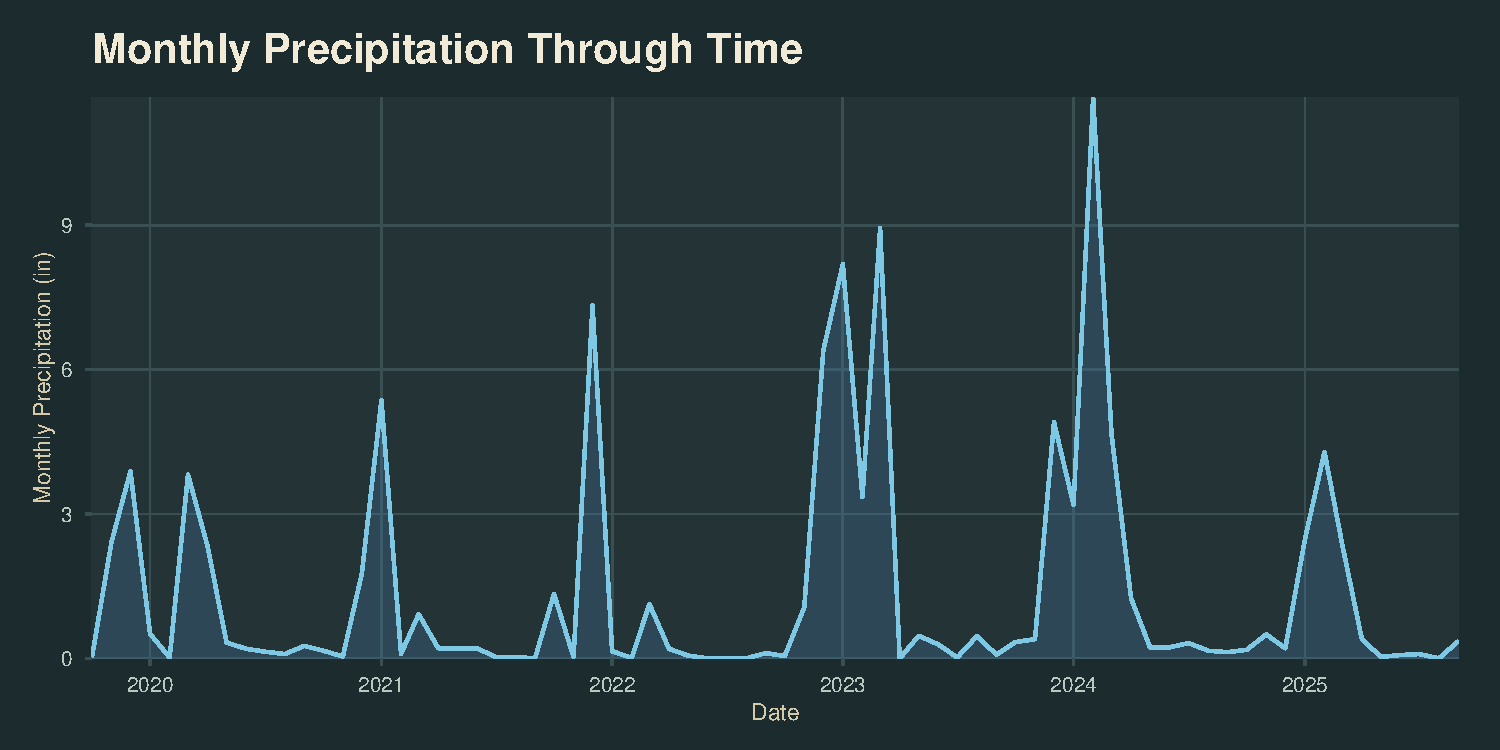
\includegraphics[keepaspectratio]{Timeline_check_in_files/figure-pdf/figure-1-precipitation-1.pdf}}

Figure 1 depicts total monthly precipitation (inches) at NCOS from water
years 2020--2025, where the shaded area and line represent total
precipitation summed across all days in each month. Precipitation
follows a strongly seasonal pattern, peaking in winter months and
dropping to near zero in summer. This figure provides environmental
context for interpreting waterfowl abundance patterns, as precipitation
may influence habitat conditions at NCOS.

\subsection{Figure 2: Monthly waterfowl abundance through time by
species}\label{figure-2-monthly-waterfowl-abundance-through-time-by-species}

\begin{Shaded}
\begin{Highlighting}[]
\CommentTok{\# color palette for all 19 species}
\NormalTok{waterfowl\_colors }\OtherTok{\textless{}{-}} \FunctionTok{c}\NormalTok{(}
  \StringTok{"American Wigeon"}             \OtherTok{=} \StringTok{"\#C1440E"}\NormalTok{,}
  \StringTok{"Blue{-}winged Teal"}            \OtherTok{=} \StringTok{"\#1B6CA8"}\NormalTok{,}
  \StringTok{"Bufflehead"}                  \OtherTok{=} \StringTok{"\#E8A838"}\NormalTok{,}
  \StringTok{"Cackling Goose (Aleutian)"}   \OtherTok{=} \StringTok{"\#9DBF9E"}\NormalTok{,}
  \StringTok{"Canada Goose"}                \OtherTok{=} \StringTok{"\#6B8E23"}\NormalTok{,}
  \StringTok{"Canvasback"}                  \OtherTok{=} \StringTok{"\#B22222"}\NormalTok{,}
  \StringTok{"Cinnamon Teal"}               \OtherTok{=} \StringTok{"\#A0522D"}\NormalTok{,}
  \StringTok{"Gadwall"}                     \OtherTok{=} \StringTok{"\#8FBC8F"}\NormalTok{,}
  \StringTok{"Greater White{-}fronted Goose"} \OtherTok{=} \StringTok{"\#D2B48C"}\NormalTok{,}
  \StringTok{"Green{-}winged Teal"}           \OtherTok{=} \StringTok{"\#2E8B57"}\NormalTok{,}
  \StringTok{"Hooded Merganser"}            \OtherTok{=} \StringTok{"\#20B2AA"}\NormalTok{,}
  \StringTok{"Mallard"}                     \OtherTok{=} \StringTok{"\#4682B4"}\NormalTok{,}
  \StringTok{"Northern Pintail"}            \OtherTok{=} \StringTok{"\#5F9EA0"}\NormalTok{,}
  \StringTok{"Northern Shoveler"}           \OtherTok{=} \StringTok{"\#3CB371"}\NormalTok{,}
  \StringTok{"Redhead"}                     \OtherTok{=} \StringTok{"\#8B1A1A"}\NormalTok{,}
  \StringTok{"Ring{-}necked Duck"}            \OtherTok{=} \StringTok{"\#6A5ACD"}\NormalTok{,}
  \StringTok{"Ross\textquotesingle{}s Goose"}                \OtherTok{=} \StringTok{"\#F4E4B8"}\NormalTok{,}
  \StringTok{"Ruddy Duck"}                  \OtherTok{=} \StringTok{"\#CD853F"}\NormalTok{,}
  \StringTok{"Snow Goose"}                  \OtherTok{=} \StringTok{"\#B0C4DE"}
\NormalTok{)}

\FunctionTok{ggplot}\NormalTok{(}\AttributeTok{data =}\NormalTok{ monthly\_waterfowl,}
       \AttributeTok{mapping =} \FunctionTok{aes}\NormalTok{(}\AttributeTok{x =}\NormalTok{ month,}
                     \AttributeTok{y =}\NormalTok{ abundance,}
                     \AttributeTok{fill =}\NormalTok{ species)) }\SpecialCharTok{+}

  \CommentTok{\# border lines between layers to reduce muddiness}
  \FunctionTok{geom\_area}\NormalTok{(}\AttributeTok{color =} \StringTok{"\#1C2B2D"}\NormalTok{, }\AttributeTok{linewidth =} \FloatTok{0.15}\NormalTok{, }\AttributeTok{alpha =} \FloatTok{0.92}\NormalTok{) }\SpecialCharTok{+}

  \FunctionTok{scale\_fill\_manual}\NormalTok{(}\AttributeTok{values =}\NormalTok{ waterfowl\_colors) }\SpecialCharTok{+}

  \FunctionTok{scale\_x\_date}\NormalTok{(}
    \AttributeTok{date\_breaks =} \StringTok{"1 year"}\NormalTok{,}
    \AttributeTok{date\_labels =} \StringTok{"\%Y"}\NormalTok{,}
    \AttributeTok{expand =} \FunctionTok{c}\NormalTok{(}\DecValTok{0}\NormalTok{, }\DecValTok{0}\NormalTok{)}
\NormalTok{  ) }\SpecialCharTok{+}

  \FunctionTok{scale\_y\_continuous}\NormalTok{(}\AttributeTok{expand =} \FunctionTok{c}\NormalTok{(}\DecValTok{0}\NormalTok{, }\DecValTok{0}\NormalTok{)) }\SpecialCharTok{+}

  \FunctionTok{labs}\NormalTok{(}
    \AttributeTok{title =} \StringTok{"Monthly Waterfowl Abundance Through Time"}\NormalTok{,}
    \AttributeTok{x     =} \StringTok{"Date"}\NormalTok{,}
    \AttributeTok{y     =} \StringTok{"Monthly Abundance (individuals)"}\NormalTok{,}
    \AttributeTok{fill  =} \ConstantTok{NULL}\NormalTok{,}
    \CommentTok{\# note the large GWFG flock count for transparency}
    \AttributeTok{caption =} \StringTok{"Note: the January 2023 peak includes a single{-}point count of 91}
\StringTok{Greater White{-}fronted Geese — a plausible but unusually large flock for this site."}
\NormalTok{  ) }\SpecialCharTok{+}

  \FunctionTok{theme\_minimal}\NormalTok{(}\AttributeTok{base\_size =} \DecValTok{13}\NormalTok{) }\SpecialCharTok{+}
  \FunctionTok{theme}\NormalTok{(}
    \AttributeTok{plot.background  =} \FunctionTok{element\_rect}\NormalTok{(}\AttributeTok{fill =} \StringTok{"\#1C2B2D"}\NormalTok{, }\AttributeTok{color =} \ConstantTok{NA}\NormalTok{),}
    \AttributeTok{panel.background =} \FunctionTok{element\_rect}\NormalTok{(}\AttributeTok{fill =} \StringTok{"\#243336"}\NormalTok{, }\AttributeTok{color =} \ConstantTok{NA}\NormalTok{),}
    \AttributeTok{panel.grid.major =} \FunctionTok{element\_line}\NormalTok{(}\AttributeTok{color =} \StringTok{"\#3A4F52"}\NormalTok{, }\AttributeTok{linewidth =} \FloatTok{0.4}\NormalTok{),}
    \AttributeTok{panel.grid.minor =} \FunctionTok{element\_blank}\NormalTok{(),}
    \AttributeTok{plot.title   =} \FunctionTok{element\_text}\NormalTok{(}\AttributeTok{color =} \StringTok{"\#F0EAD6"}\NormalTok{, }\AttributeTok{size =} \DecValTok{20}\NormalTok{, }\AttributeTok{face =} \StringTok{"bold"}\NormalTok{,}
                                \AttributeTok{margin =} \FunctionTok{margin}\NormalTok{(}\AttributeTok{b =} \DecValTok{12}\NormalTok{), }\AttributeTok{hjust =} \DecValTok{0}\NormalTok{),}
    \AttributeTok{plot.caption =} \FunctionTok{element\_text}\NormalTok{(}\AttributeTok{color =} \StringTok{"\#7A9A95"}\NormalTok{, }\AttributeTok{size =} \DecValTok{8}\NormalTok{, }\AttributeTok{hjust =} \DecValTok{0}\NormalTok{,}
                                \AttributeTok{margin =} \FunctionTok{margin}\NormalTok{(}\AttributeTok{t =} \DecValTok{8}\NormalTok{)),}
    \AttributeTok{axis.text    =} \FunctionTok{element\_text}\NormalTok{(}\AttributeTok{color =} \StringTok{"\#B8C9C2"}\NormalTok{, }\AttributeTok{size =} \DecValTok{10}\NormalTok{),}
    \AttributeTok{axis.title   =} \FunctionTok{element\_text}\NormalTok{(}\AttributeTok{color =} \StringTok{"\#D4C9A8"}\NormalTok{, }\AttributeTok{size =} \DecValTok{11}\NormalTok{),}
    \AttributeTok{axis.ticks   =} \FunctionTok{element\_line}\NormalTok{(}\AttributeTok{color =} \StringTok{"\#3A4F52"}\NormalTok{),}
    \AttributeTok{legend.position   =} \StringTok{"right"}\NormalTok{,}
    \AttributeTok{legend.background =} \FunctionTok{element\_rect}\NormalTok{(}\AttributeTok{fill =} \StringTok{"\#1C2B2D"}\NormalTok{, }\AttributeTok{color =} \ConstantTok{NA}\NormalTok{),}
    \AttributeTok{legend.key        =} \FunctionTok{element\_rect}\NormalTok{(}\AttributeTok{fill =} \ConstantTok{NA}\NormalTok{, }\AttributeTok{color =} \ConstantTok{NA}\NormalTok{),}
    \AttributeTok{legend.text       =} \FunctionTok{element\_text}\NormalTok{(}\AttributeTok{color =} \StringTok{"\#F0EAD6"}\NormalTok{, }\AttributeTok{size =} \FloatTok{8.5}\NormalTok{),}
    \AttributeTok{legend.key.size   =} \FunctionTok{unit}\NormalTok{(}\FloatTok{0.45}\NormalTok{, }\StringTok{"cm"}\NormalTok{),}
    \AttributeTok{legend.spacing.y  =} \FunctionTok{unit}\NormalTok{(}\FloatTok{0.1}\NormalTok{, }\StringTok{"cm"}\NormalTok{),}
    \AttributeTok{plot.margin =} \FunctionTok{margin}\NormalTok{(}\DecValTok{16}\NormalTok{, }\DecValTok{20}\NormalTok{, }\DecValTok{12}\NormalTok{, }\DecValTok{16}\NormalTok{)}
\NormalTok{  )}
\end{Highlighting}
\end{Shaded}

\pandocbounded{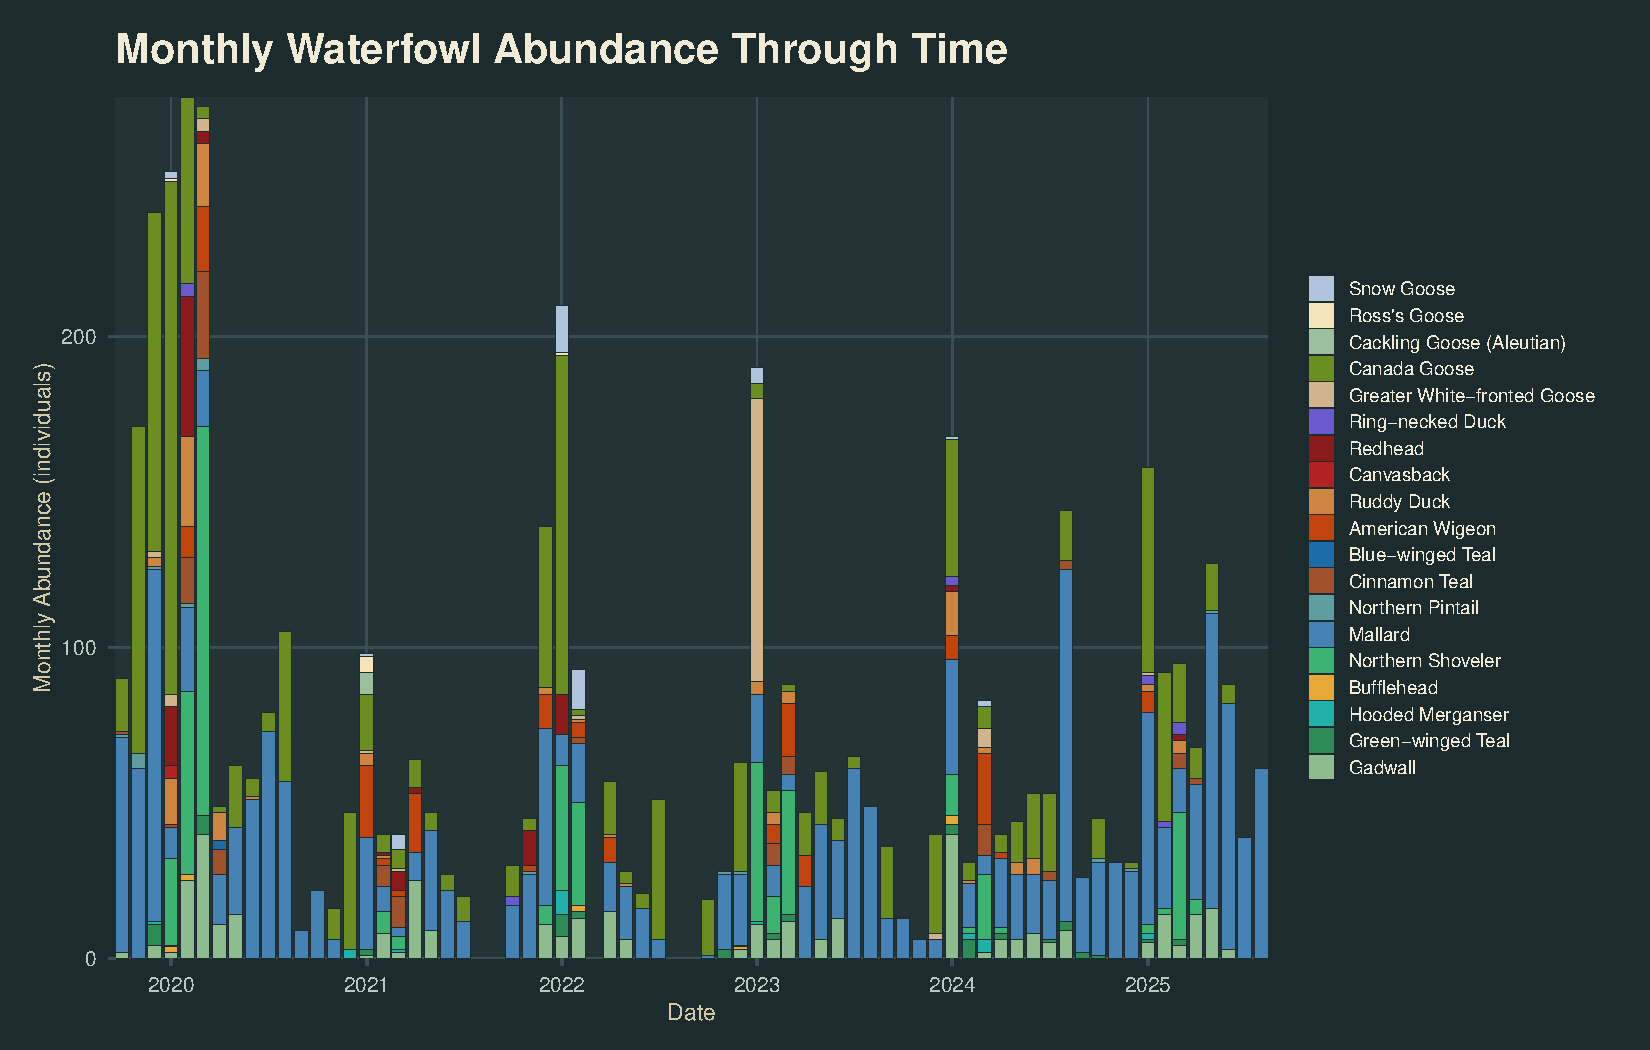
\includegraphics[keepaspectratio]{Timeline_check_in_files/figure-pdf/figure-2-waterfowl-1.pdf}}

Figure 2 depicts total monthly waterfowl abundance at NCOS from water
years 2020--2025, where each colored layer represents the summed monthly
count of one waterfowl species, stacked to show total abundance across
all species. Note: three species (Blue-winged Teal, Cackling Goose
(Aleutian), Canvasback) are present in the data set but not visible due
to very low counts (≤7 individuals total). Abundance is highest in early
2020 and generally declines through the study period, with peaks
concentrated in winter months. This figure directly addresses our
question of how waterfowl abundance varies through time at NCOS.

\subsection{Figure 3: Figure 3: Lagged precipitation vs.~total waterfowl
abundance}\label{figure-3-figure-3-lagged-precipitation-vs.-total-waterfowl-abundance}

\begin{Shaded}
\begin{Highlighting}[]
\FunctionTok{ggplot}\NormalTok{(}\AttributeTok{data =}\NormalTok{ bird\_weather\_monthly,}
       \AttributeTok{mapping =} \FunctionTok{aes}\NormalTok{(}\AttributeTok{x =}\NormalTok{ lagged\_prcp,}
                     \AttributeTok{y =}\NormalTok{ total\_abundance,}
                     \CommentTok{\# color by month of year (1{-}12) to show seasonal patterns}
                     \AttributeTok{color =}\NormalTok{ month\_of\_year)) }\SpecialCharTok{+}

  \FunctionTok{geom\_point}\NormalTok{(}\AttributeTok{alpha =} \FloatTok{0.85}\NormalTok{, }\AttributeTok{size =} \DecValTok{4}\NormalTok{) }\SpecialCharTok{+}

  \FunctionTok{scale\_color\_viridis\_c}\NormalTok{(}
    \AttributeTok{name   =} \StringTok{"Month"}\NormalTok{,}
    \AttributeTok{option =} \StringTok{"turbo"}\NormalTok{,}
    \AttributeTok{breaks =} \FunctionTok{c}\NormalTok{(}\DecValTok{1}\NormalTok{, }\DecValTok{3}\NormalTok{, }\DecValTok{5}\NormalTok{, }\DecValTok{7}\NormalTok{, }\DecValTok{9}\NormalTok{, }\DecValTok{11}\NormalTok{),}
    \AttributeTok{labels =} \FunctionTok{c}\NormalTok{(}\StringTok{"Jan"}\NormalTok{, }\StringTok{"Mar"}\NormalTok{, }\StringTok{"May"}\NormalTok{, }\StringTok{"Jul"}\NormalTok{, }\StringTok{"Sep"}\NormalTok{, }\StringTok{"Nov"}\NormalTok{),}
    \AttributeTok{limits =} \FunctionTok{c}\NormalTok{(}\DecValTok{1}\NormalTok{, }\DecValTok{12}\NormalTok{)}
\NormalTok{  ) }\SpecialCharTok{+}

  \FunctionTok{labs}\NormalTok{(}
    \AttributeTok{title   =} \StringTok{"Relationship Between Precipitation and Waterfowl Abundance"}\NormalTok{,}
    \AttributeTok{x       =} \StringTok{"Previous Month\textquotesingle{}s Precipitation (in)"}\NormalTok{,}
    \AttributeTok{y       =} \StringTok{"Total Monthly Waterfowl Abundance (individuals)"}\NormalTok{,}
    \AttributeTok{caption =} \StringTok{"Each point represents one month\textquotesingle{}s waterfowl abundance plotted}
\StringTok{against the previous month\textquotesingle{}s precipitation. Points colored by month of year."}
\NormalTok{  ) }\SpecialCharTok{+}

  \FunctionTok{theme\_minimal}\NormalTok{(}\AttributeTok{base\_size =} \DecValTok{13}\NormalTok{) }\SpecialCharTok{+}
  \FunctionTok{theme}\NormalTok{(}
    \AttributeTok{plot.background  =} \FunctionTok{element\_rect}\NormalTok{(}\AttributeTok{fill =} \StringTok{"\#1C2B2D"}\NormalTok{, }\AttributeTok{color =} \ConstantTok{NA}\NormalTok{),}
    \AttributeTok{panel.background =} \FunctionTok{element\_rect}\NormalTok{(}\AttributeTok{fill =} \StringTok{"\#243336"}\NormalTok{, }\AttributeTok{color =} \ConstantTok{NA}\NormalTok{),}
    \AttributeTok{panel.grid.major =} \FunctionTok{element\_line}\NormalTok{(}\AttributeTok{color =} \StringTok{"\#3A4F52"}\NormalTok{, }\AttributeTok{linewidth =} \FloatTok{0.4}\NormalTok{),}
    \AttributeTok{panel.grid.minor =} \FunctionTok{element\_blank}\NormalTok{(),}
    \AttributeTok{plot.title   =} \FunctionTok{element\_text}\NormalTok{(}\AttributeTok{color =} \StringTok{"\#F0EAD6"}\NormalTok{, }\AttributeTok{size =} \DecValTok{20}\NormalTok{, }\AttributeTok{face =} \StringTok{"bold"}\NormalTok{,}
                                \AttributeTok{margin =} \FunctionTok{margin}\NormalTok{(}\AttributeTok{b =} \DecValTok{12}\NormalTok{), }\AttributeTok{hjust =} \DecValTok{0}\NormalTok{),}
    \AttributeTok{plot.caption =} \FunctionTok{element\_text}\NormalTok{(}\AttributeTok{color =} \StringTok{"\#7A9A95"}\NormalTok{, }\AttributeTok{size =} \FloatTok{8.5}\NormalTok{, }\AttributeTok{hjust =} \DecValTok{0}\NormalTok{,}
                                \AttributeTok{margin =} \FunctionTok{margin}\NormalTok{(}\AttributeTok{t =} \DecValTok{8}\NormalTok{)),}
    \AttributeTok{axis.text    =} \FunctionTok{element\_text}\NormalTok{(}\AttributeTok{color =} \StringTok{"\#B8C9C2"}\NormalTok{, }\AttributeTok{size =} \DecValTok{10}\NormalTok{),}
    \AttributeTok{axis.title   =} \FunctionTok{element\_text}\NormalTok{(}\AttributeTok{color =} \StringTok{"\#D4C9A8"}\NormalTok{, }\AttributeTok{size =} \DecValTok{11}\NormalTok{),}
    \AttributeTok{axis.ticks   =} \FunctionTok{element\_line}\NormalTok{(}\AttributeTok{color =} \StringTok{"\#3A4F52"}\NormalTok{),}
    \AttributeTok{legend.background =} \FunctionTok{element\_rect}\NormalTok{(}\AttributeTok{fill =} \StringTok{"\#1C2B2D"}\NormalTok{, }\AttributeTok{color =} \ConstantTok{NA}\NormalTok{),}
    \AttributeTok{legend.key        =} \FunctionTok{element\_rect}\NormalTok{(}\AttributeTok{fill =} \ConstantTok{NA}\NormalTok{, }\AttributeTok{color =} \ConstantTok{NA}\NormalTok{),}
    \AttributeTok{legend.text       =} \FunctionTok{element\_text}\NormalTok{(}\AttributeTok{color =} \StringTok{"\#F0EAD6"}\NormalTok{, }\AttributeTok{size =} \DecValTok{9}\NormalTok{),}
    \AttributeTok{legend.title      =} \FunctionTok{element\_text}\NormalTok{(}\AttributeTok{color =} \StringTok{"\#D4C9A8"}\NormalTok{, }\AttributeTok{size =} \DecValTok{10}\NormalTok{, }\AttributeTok{face =} \StringTok{"bold"}\NormalTok{),}
    \AttributeTok{legend.key.height =} \FunctionTok{unit}\NormalTok{(}\FloatTok{1.2}\NormalTok{, }\StringTok{"cm"}\NormalTok{),}
    \AttributeTok{plot.margin =} \FunctionTok{margin}\NormalTok{(}\DecValTok{16}\NormalTok{, }\DecValTok{20}\NormalTok{, }\DecValTok{12}\NormalTok{, }\DecValTok{16}\NormalTok{)}
\NormalTok{  )}
\end{Highlighting}
\end{Shaded}

\pandocbounded{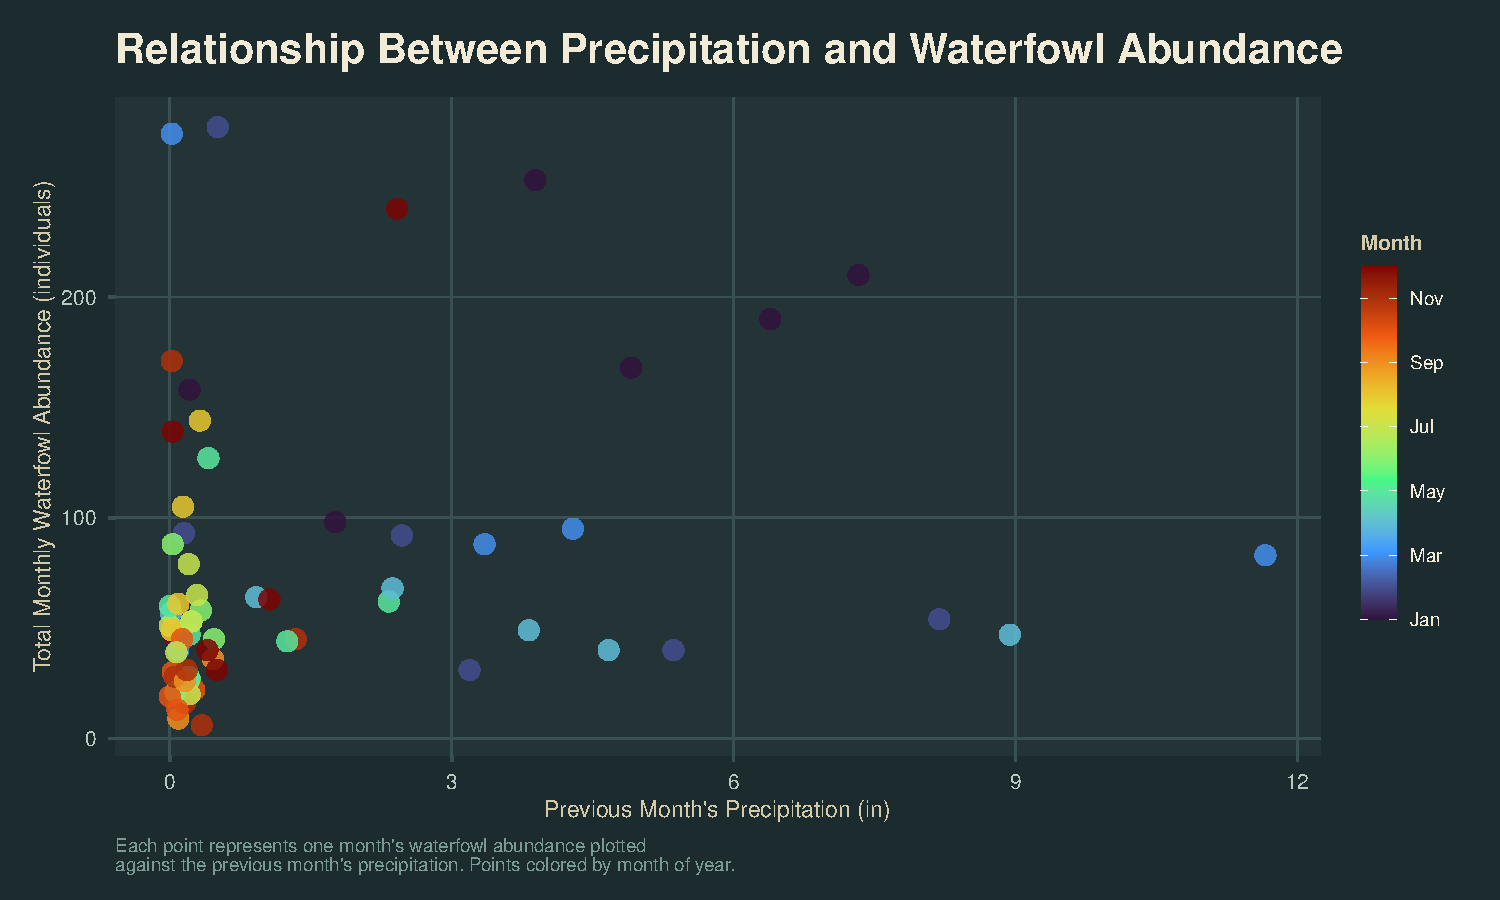
\includegraphics[keepaspectratio]{Timeline_check_in_files/figure-pdf/figure-3-lagged-precip-1.pdf}}

Figure 3 depicts the relationship between total monthly waterfowl
abundance and the previous month's total precipitation at NCOS from
water years 2020--2025, where each point represents one month colored by
month of year. The figure shows no clear linear trend between lagged
precipitation and waterfowl abundance, suggesting that the previous
month's precipitation does not strongly predict waterfowl abundance at
NCOS. This figure directly addresses our primary research question about
the effect of precipitation on waterfowl abundance.

\section{Other exploratory
visualizations}\label{other-exploratory-visualizations}

\subsection{Figure 4: Average seasonal trends comparing waterfowl
abundance and
precipitation}\label{figure-4-average-seasonal-trends-comparing-waterfowl-abundance-and-precipitation}

\begin{Shaded}
\begin{Highlighting}[]
\CommentTok{\# shared theme}
\NormalTok{seasonal\_theme }\OtherTok{\textless{}{-}} \FunctionTok{theme\_minimal}\NormalTok{(}\AttributeTok{base\_size =} \DecValTok{13}\NormalTok{) }\SpecialCharTok{+}
  \FunctionTok{theme}\NormalTok{(}
    \AttributeTok{plot.background  =} \FunctionTok{element\_rect}\NormalTok{(}\AttributeTok{fill =} \StringTok{"\#1C2B2D"}\NormalTok{, }\AttributeTok{color =} \ConstantTok{NA}\NormalTok{),}
    \AttributeTok{panel.background =} \FunctionTok{element\_rect}\NormalTok{(}\AttributeTok{fill =} \StringTok{"\#243336"}\NormalTok{, }\AttributeTok{color =} \ConstantTok{NA}\NormalTok{),}
    \AttributeTok{panel.grid.major =} \FunctionTok{element\_line}\NormalTok{(}\AttributeTok{color =} \StringTok{"\#3A4F52"}\NormalTok{, }\AttributeTok{linewidth =} \FloatTok{0.4}\NormalTok{),}
    \AttributeTok{panel.grid.minor =} \FunctionTok{element\_blank}\NormalTok{(),}
    \AttributeTok{plot.title  =} \FunctionTok{element\_text}\NormalTok{(}\AttributeTok{color =} \StringTok{"\#F0EAD6"}\NormalTok{, }\AttributeTok{size =} \DecValTok{14}\NormalTok{, }\AttributeTok{face =} \StringTok{"bold"}\NormalTok{,}
                               \AttributeTok{margin =} \FunctionTok{margin}\NormalTok{(}\AttributeTok{b =} \DecValTok{8}\NormalTok{), }\AttributeTok{hjust =} \DecValTok{0}\NormalTok{),}
    \AttributeTok{axis.text   =} \FunctionTok{element\_text}\NormalTok{(}\AttributeTok{color =} \StringTok{"\#B8C9C2"}\NormalTok{, }\AttributeTok{size =} \DecValTok{10}\NormalTok{),}
    \AttributeTok{axis.title  =} \FunctionTok{element\_text}\NormalTok{(}\AttributeTok{color =} \StringTok{"\#D4C9A8"}\NormalTok{, }\AttributeTok{size =} \DecValTok{11}\NormalTok{),}
    \AttributeTok{axis.ticks  =} \FunctionTok{element\_line}\NormalTok{(}\AttributeTok{color =} \StringTok{"\#3A4F52"}\NormalTok{),}
    \AttributeTok{plot.margin =} \FunctionTok{margin}\NormalTok{(}\DecValTok{12}\NormalTok{, }\DecValTok{20}\NormalTok{, }\DecValTok{8}\NormalTok{, }\DecValTok{16}\NormalTok{)}
\NormalTok{  )}

\CommentTok{\# panel A}
\NormalTok{plot\_abundance }\OtherTok{\textless{}{-}} \FunctionTok{ggplot}\NormalTok{() }\SpecialCharTok{+}
  \FunctionTok{geom\_point}\NormalTok{(}
    \AttributeTok{data     =}\NormalTok{ seasonal\_by\_year,}
    \AttributeTok{mapping  =} \FunctionTok{aes}\NormalTok{(}\AttributeTok{x =}\NormalTok{ season, }\AttributeTok{y =}\NormalTok{ seasonal\_abundance, }\AttributeTok{group =} \DecValTok{1}\NormalTok{),}
    \AttributeTok{color    =} \StringTok{"\#7EC8E3"}\NormalTok{, }\AttributeTok{alpha =} \FloatTok{0.35}\NormalTok{, }\AttributeTok{size =} \FloatTok{2.5}\NormalTok{,}
    \AttributeTok{position =} \FunctionTok{position\_jitter}\NormalTok{(}\AttributeTok{width =} \FloatTok{0.08}\NormalTok{, }\AttributeTok{seed =} \DecValTok{42}\NormalTok{)}
\NormalTok{  ) }\SpecialCharTok{+}
  \FunctionTok{geom\_line}\NormalTok{(}
    \AttributeTok{data    =}\NormalTok{ seasonal\_summary,}
    \AttributeTok{mapping =} \FunctionTok{aes}\NormalTok{(}\AttributeTok{x =}\NormalTok{ season, }\AttributeTok{y =}\NormalTok{ avg\_abundance, }\AttributeTok{group =} \DecValTok{1}\NormalTok{),}
    \AttributeTok{color =} \StringTok{"\#7EC8E3"}\NormalTok{, }\AttributeTok{linewidth =} \FloatTok{1.2}
\NormalTok{  ) }\SpecialCharTok{+}
  \FunctionTok{geom\_point}\NormalTok{(}
    \AttributeTok{data    =}\NormalTok{ seasonal\_summary,}
    \AttributeTok{mapping =} \FunctionTok{aes}\NormalTok{(}\AttributeTok{x =}\NormalTok{ season, }\AttributeTok{y =}\NormalTok{ avg\_abundance, }\AttributeTok{group =} \DecValTok{1}\NormalTok{),}
    \AttributeTok{color =} \StringTok{"\#7EC8E3"}\NormalTok{, }\AttributeTok{size =} \DecValTok{4}
\NormalTok{  ) }\SpecialCharTok{+}
  \FunctionTok{labs}\NormalTok{(}
    \AttributeTok{title =} \StringTok{"Average Total Seasonal Waterfowl Abundance"}\NormalTok{,}
    \AttributeTok{x     =} \StringTok{"Season"}\NormalTok{,}
    \AttributeTok{y     =} \StringTok{"Abundance (individuals)"}
\NormalTok{  ) }\SpecialCharTok{+}
\NormalTok{  seasonal\_theme}

\CommentTok{\# panel B}
\NormalTok{plot\_precip }\OtherTok{\textless{}{-}} \FunctionTok{ggplot}\NormalTok{() }\SpecialCharTok{+}
  \FunctionTok{geom\_point}\NormalTok{(}
    \AttributeTok{data     =}\NormalTok{ seasonal\_by\_year,}
    \AttributeTok{mapping  =} \FunctionTok{aes}\NormalTok{(}\AttributeTok{x =}\NormalTok{ season, }\AttributeTok{y =}\NormalTok{ seasonal\_prcp, }\AttributeTok{group =} \DecValTok{1}\NormalTok{),}
    \AttributeTok{color    =} \StringTok{"\#6B8E23"}\NormalTok{, }\AttributeTok{alpha =} \FloatTok{0.35}\NormalTok{, }\AttributeTok{size =} \FloatTok{2.5}\NormalTok{,}
    \AttributeTok{position =} \FunctionTok{position\_jitter}\NormalTok{(}\AttributeTok{width =} \FloatTok{0.08}\NormalTok{, }\AttributeTok{seed =} \DecValTok{42}\NormalTok{)}
\NormalTok{  ) }\SpecialCharTok{+}
  \FunctionTok{geom\_line}\NormalTok{(}
    \AttributeTok{data    =}\NormalTok{ seasonal\_summary,}
    \AttributeTok{mapping =} \FunctionTok{aes}\NormalTok{(}\AttributeTok{x =}\NormalTok{ season, }\AttributeTok{y =}\NormalTok{ avg\_prcp, }\AttributeTok{group =} \DecValTok{1}\NormalTok{),}
    \AttributeTok{color =} \StringTok{"\#6B8E23"}\NormalTok{, }\AttributeTok{linewidth =} \FloatTok{1.2}
\NormalTok{  ) }\SpecialCharTok{+}
  \FunctionTok{geom\_point}\NormalTok{(}
    \AttributeTok{data    =}\NormalTok{ seasonal\_summary,}
    \AttributeTok{mapping =} \FunctionTok{aes}\NormalTok{(}\AttributeTok{x =}\NormalTok{ season, }\AttributeTok{y =}\NormalTok{ avg\_prcp, }\AttributeTok{group =} \DecValTok{1}\NormalTok{),}
    \AttributeTok{color =} \StringTok{"\#6B8E23"}\NormalTok{, }\AttributeTok{size =} \DecValTok{4}
\NormalTok{  ) }\SpecialCharTok{+}
  \FunctionTok{labs}\NormalTok{(}
    \AttributeTok{title =} \StringTok{"Average Total Seasonal Precipitation"}\NormalTok{,}
    \AttributeTok{x     =} \StringTok{"Season"}\NormalTok{,}
    \AttributeTok{y     =} \StringTok{"Precipitation (in)"}
\NormalTok{  ) }\SpecialCharTok{+}
\NormalTok{  seasonal\_theme}

\CommentTok{\# combine}
\NormalTok{combined\_plot }\OtherTok{\textless{}{-}}\NormalTok{ (plot\_abundance }\SpecialCharTok{/}\NormalTok{ plot\_precip) }\SpecialCharTok{+}
  \FunctionTok{plot\_annotation}\NormalTok{(}
    \AttributeTok{title   =} \StringTok{"Seasonal Patterns in Waterfowl Abundance and Precipitation"}\NormalTok{,}
    \AttributeTok{caption =} \StringTok{"Points show individual water{-}year seasonal totals; lines show averages across water years 2020{-}2025."}\NormalTok{,}
    \AttributeTok{theme   =} \FunctionTok{theme}\NormalTok{(}
      \AttributeTok{plot.background =} \FunctionTok{element\_rect}\NormalTok{(}\AttributeTok{fill =} \StringTok{"\#1C2B2D"}\NormalTok{, }\AttributeTok{color =} \ConstantTok{NA}\NormalTok{),}
      \AttributeTok{plot.title      =} \FunctionTok{element\_text}\NormalTok{(}\AttributeTok{color =} \StringTok{"\#F0EAD6"}\NormalTok{, }\AttributeTok{size =} \DecValTok{18}\NormalTok{, }\AttributeTok{face =} \StringTok{"bold"}\NormalTok{,}
                                     \AttributeTok{hjust =} \DecValTok{0}\NormalTok{, }\AttributeTok{margin =} \FunctionTok{margin}\NormalTok{(}\AttributeTok{b =} \DecValTok{10}\NormalTok{)),}
      \AttributeTok{plot.caption    =} \FunctionTok{element\_text}\NormalTok{(}\AttributeTok{color =} \StringTok{"\#7A9A95"}\NormalTok{, }\AttributeTok{size =} \FloatTok{8.5}\NormalTok{, }\AttributeTok{hjust =} \DecValTok{0}\NormalTok{,}
                                     \AttributeTok{margin =} \FunctionTok{margin}\NormalTok{(}\AttributeTok{t =} \DecValTok{8}\NormalTok{))}
\NormalTok{    )}
\NormalTok{  )}

\NormalTok{combined\_plot}
\end{Highlighting}
\end{Shaded}

\pandocbounded{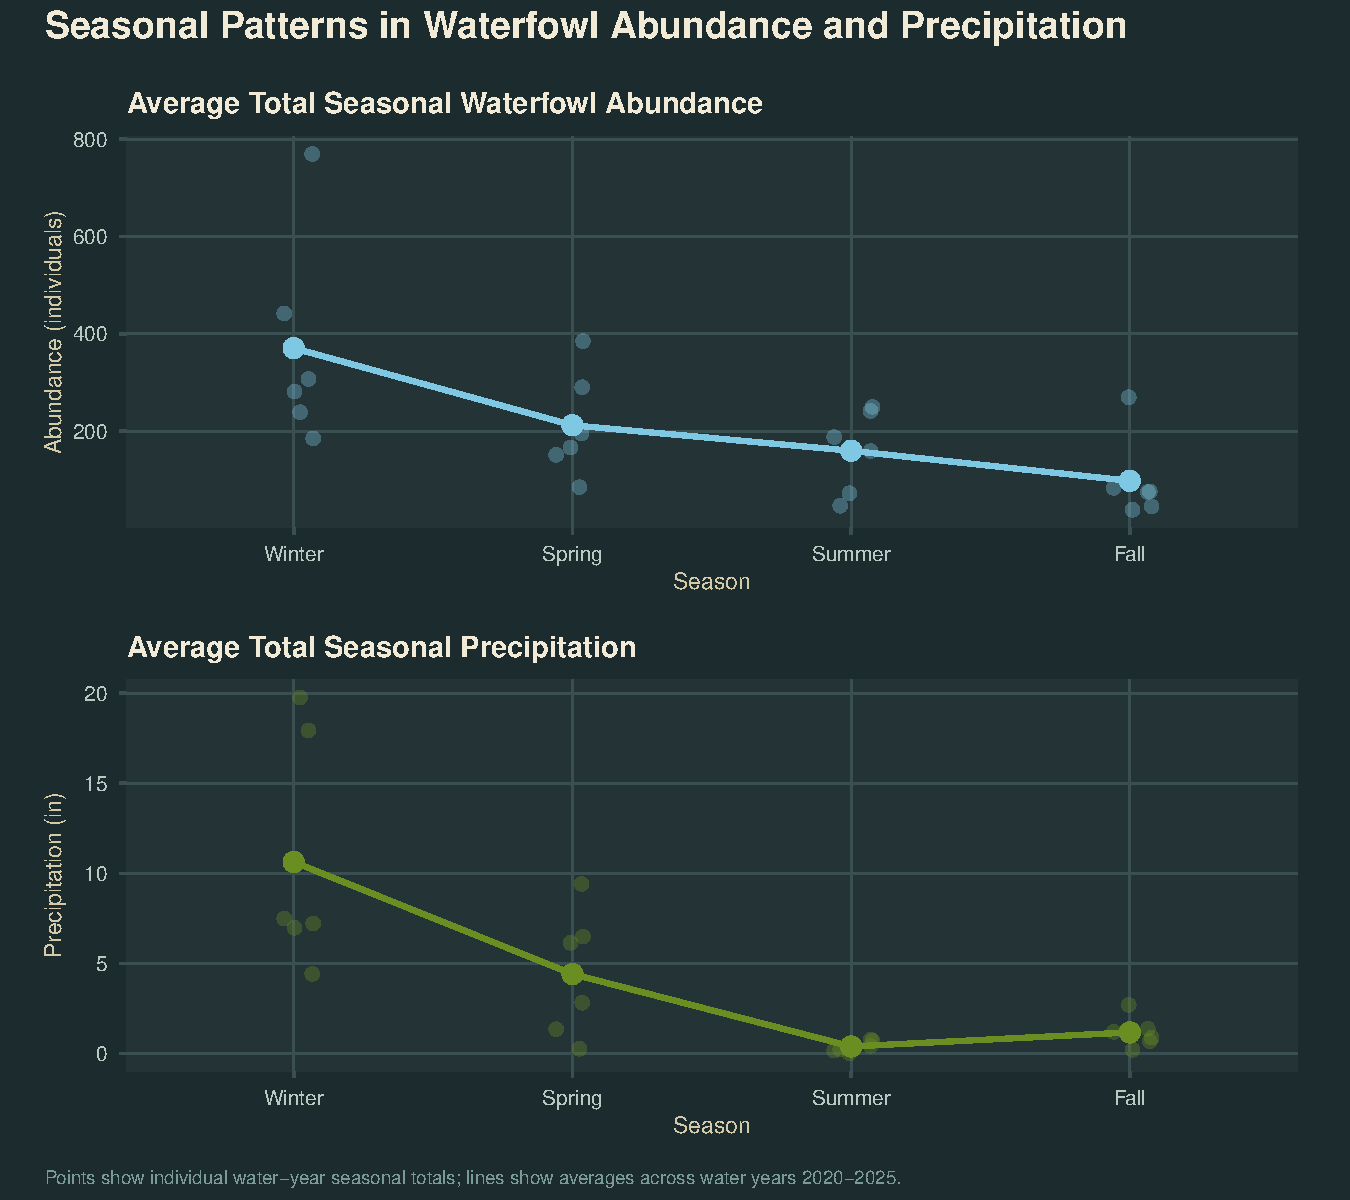
\includegraphics[keepaspectratio]{Timeline_check_in_files/figure-pdf/figure-4-seasonal-abundance-precip-1.pdf}}

Figure 4 uses two stacked panels to compare average total seasonal
waterfowl abundance and average total seasonal precipitation across
water years 2020-2025. Small points show individual water-year seasonal
totals to display the spread of observations; larger points and lines
show the average across all water years. Both variables are highest in
winter and lowest in summer, suggesting that waterfowl and precipitation
follow similar seasonal patterns. However, Figure 3 indicates this
parallel trend does not reflect a direct causal relationship. This
figure contextualizes our main question by showing that seasonal timing,
rather than precipitation amount, may better explain patterns in
waterfowl abundance at NCOS.

\section{Plan for elective}\label{plan-for-elective}

\subsection{Conecpt}\label{conecpt}

We want to create a tangible brochure to be available along the NCOS
trail. It will serve as a visitor's guide to waterfowl spotting,
featuring the most prevalent of our 19 waterfowl species observed in the
dataset.

\subsection{Proposed Layout}\label{proposed-layout}

\begin{itemize}
\item
  \textbf{``Species profiles:} Small illustrations or photos, a fun
  fact, and best time of year to spot the species based on our data
\item
  \textbf{``When to Visit'' guide:} A seasonal breakdown of which
  species are most abundant, informed by figure 4.
\item
  \textbf{Precipitation Note:} A fun callout illustrating which species
  are most active during rainy seasons, tying in our findings.
\end{itemize}

\subsection{Two-Week Plan}\label{two-week-plan}

\begin{itemize}
\item
  \textbf{Week 1:} Finalize brochure layout and species selection,
  gather create illustrations of species, draft facts and relevant data.
\item
  \textbf{Week 2:} Design Brochure in Canva, incorporating figures from
  our analysis, review and finalize for print.
\end{itemize}

\subsection{Brochure Blueprint}\label{brochure-blueprint}

\begin{figure}[H]

{\centering \pandocbounded{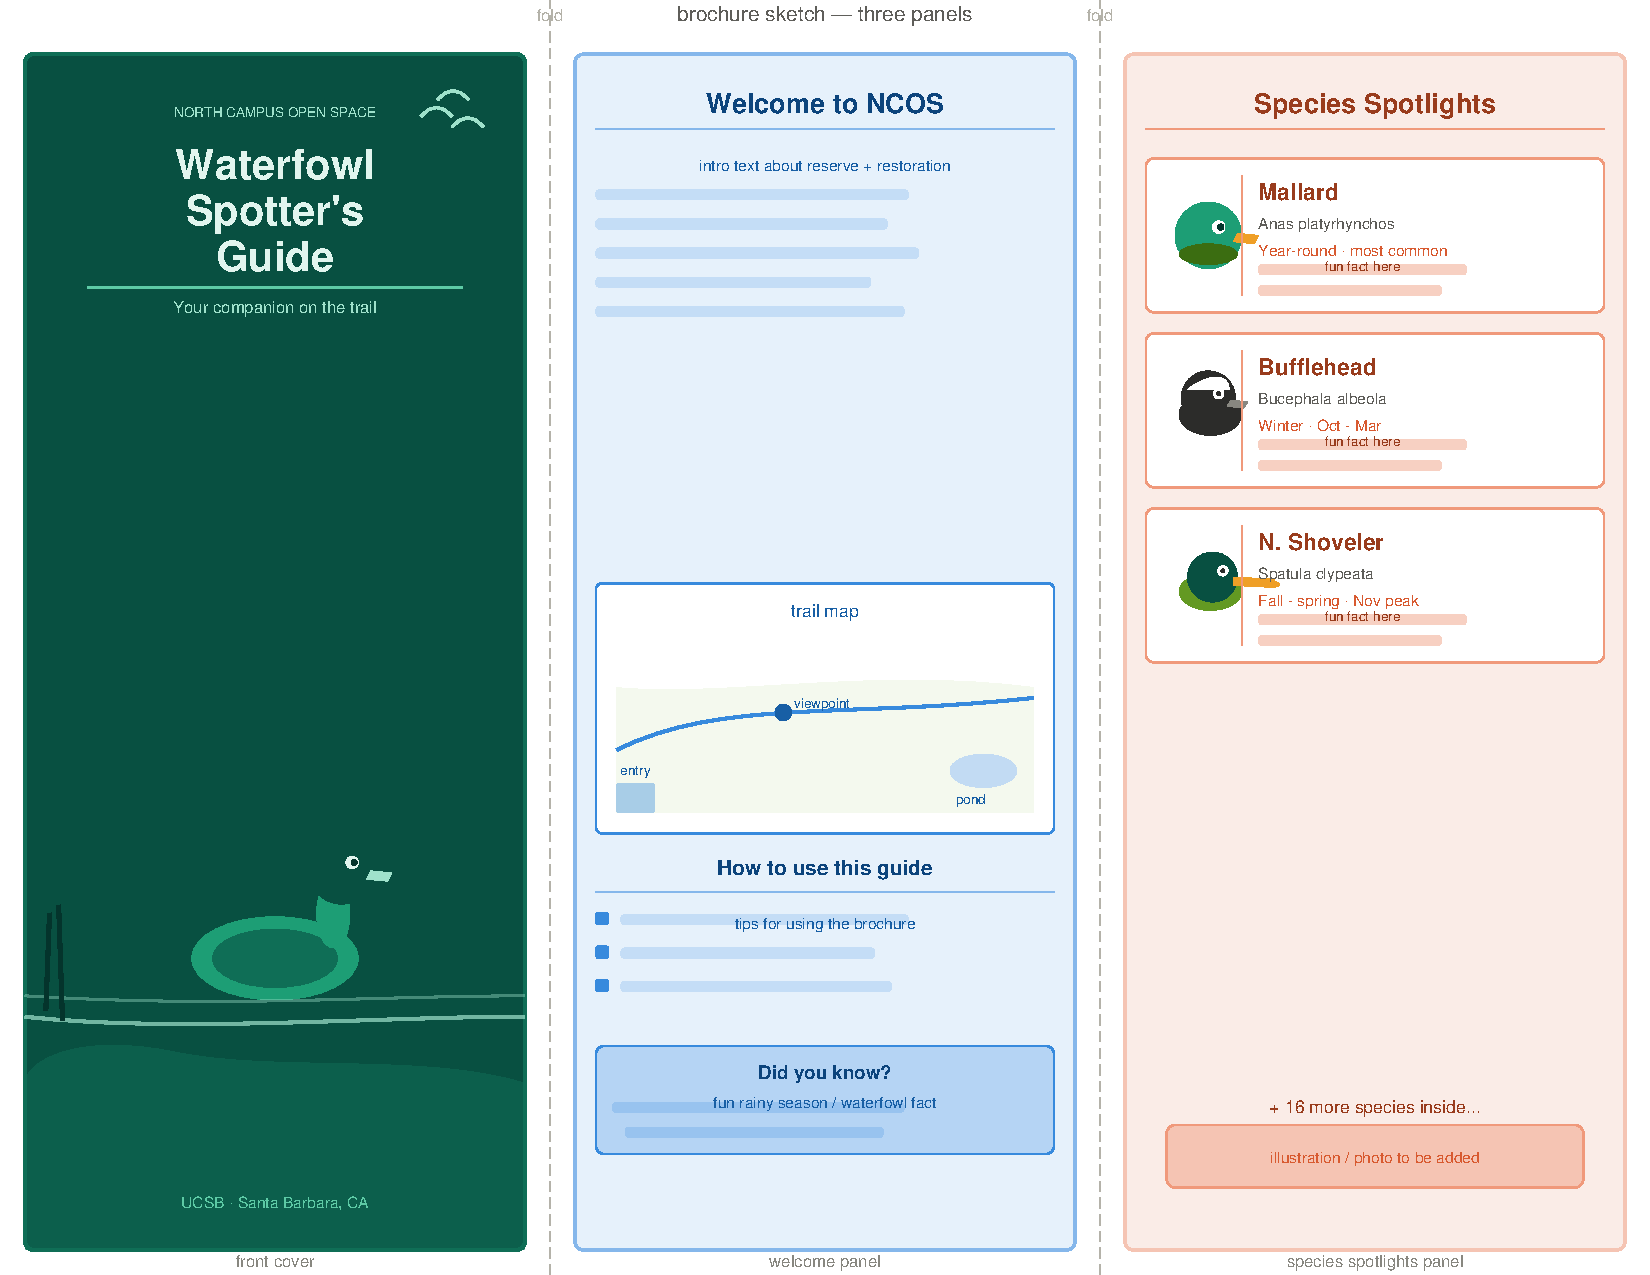
\includegraphics[keepaspectratio]{figures/brochure-draft.pdf}}

}

\caption{Brochure draft sketch}

\end{figure}%

\phantomsection\label{refs}
\begin{CSLReferences}{1}{0}
\bibitem[\citeproctext]{ref-kahara2021}
Kahara, Sharon N., Daniel Skalos, Buddhika Madurapperuma, and Kaitlyn
Hernandez. 2021. {``Habitat Quality and Drought Effects on Breeding
Mallard and Other Waterfowl Populations in California, USA.''} \emph{The
Journal of Wildlife Management} 86 (1).
\url{https://doi.org/10.1002/jwmg.22133}.

\bibitem[\citeproctext]{ref-stenzel2011}
Stenzel, Lynne E., and Gary W. Page. 2011. {``Trends in Abundance of
Wintering Waterbirds Relative to Rainfall Patterns at a Central
California Estuary, 1972-2015.''} \emph{Western Birds}.
\url{https://doi.org/10.21199/SWB3.13}.

\bibitem[\citeproctext]{ref-withey2011}
Withey, Patrick, and G. Cornelis van Kooten. 2011. {``The Effect of
Climate Change on Optimal Wetlands and Waterfowl Management in Western
Canada.''} \emph{Ecological Economics} 70 (4): 798--805.
\url{https://doi.org/10.1016/j.ecolecon.2010.11.019}.

\bibitem[\citeproctext]{ref-zhao2016}
Zhao, Qing, Emily Silverman, Kathy Fleming, and G. Scott Boomer. 2016.
{``Forecasting Waterfowl Population Dynamics Under Climate Change
{\textemdash} Does the Spatial Variation of Density Dependence and
Environmental Effects Matter?''} \emph{Biological Conservation} 194
(February): 80--88. \url{https://doi.org/10.1016/j.biocon.2015.12.006}.

\end{CSLReferences}




\end{document}
